\chapter{Исследовательская часть}

\section{Технические характеристики}
Характеристики используемого оборудования:
\begin{itemize}
    \item Операционная система --- Windows 11 Home [5]
    \item Память --- 16 Гб.
    \item Процессор --- Intel(R) Core(TM) i5-10300H CPU @ 2.50ГГц [6]
\end{itemize}

\section{Описание используемых типов данных}
Используемые типы данных:
\begin{itemize}
	\item строка --- последовательность символов типа $str$;
	\item длина строки --- целое число типа $int$;
	\item матрица --- двумерный массив типа $int$.
\end{itemize}

\section{Оценка памяти}

Рекурсивная версия алгоритма Левенштейна не использует явных структур данных для хранения промежуточных вычислений. Вместо этого каждый вызов функции обрабатывает небольшой фрагмент строк, и функция вызывает саму себя несколько раз. Глубина рекурсии в худшем случае составляет: 
\begin{equation}
	(len(S_{1}) + len(S_{2})).
\end{equation}
При этом каждый рекурсивный вызов требует хранения локальных переменных: 2 переменные типа $int$, 2 переменные типа $str$. В результате, максимальный расход памяти составляет:
\begin{equation}
	(len(S_{1}) + len(S_{2})) \cdot (2 \cdot size(\text{int}) + 2 \cdot size(\text{str})),
\end{equation}
где $size$ - функция, вычисляющая размер параметра.

Алгоритм, основанный на динамическом программировании, использует двумерную матрицу размером $len(S_{1} + 1) \times len(S_{2} + 1)$
Эта матрица хранит результаты всех промежуточных вычислений (расстояние Левенштейна для всех подстрок). Дополнительно хранятся локальные переменные: 5 переменных типа $int$, 2 переменные типа $str$. По итогу расход памяти в данном случае составляет:
\begin{equation}
	(len(S_{1} + 1) \cdot len(S_{2} + 1) \cdot size(\text{int})) + 5 \cdot size(\text{int}) + 2 \cdot size(\text{str})).
\end{equation}

По расходу памяти алгоритм, использующий принцип динамического программирования, проигрывает рекурсивному: максимальный размер используемой памяти в них растёт как произведение длин строк, в то время как у рекурсивного алгоритма — как сумма длин строк.

Алгоритм Дамерау-Левенштейна, также реализованный через динамическое программирование, аналогичен по своей структуре алгоритму Левенштейна. Основное отличие заключается в дополнительной проверке для учёта операций перестановки соседних символов. Для этого используется та же матрица размера 
$len(S_{1} + 1) \times (len(S_{2} + 1)$
, что и в динамическом алгоритме Левенштейна.

Несмотря на добавление новой операции (перестановка), использование памяти остаётся также на уровне 
произведение длин строк, поскольку не требуется дополнительное пространство для хранения результатов перестановок. Как и в случае с Левенштейном, каждая клетка матрицы заполняется лишь однажды.

\clearpage

\section{Время выполнения алгоритмов}
Результаты замеров времени работы алгоритмов нахождения расстояний Левенштейна и Дамерау–Левенштейна приведены в таблице \ref{tbl:time_measurements}. На рисунке \ref{fig:time_measurements} приведены графики зависимости времени от количества букв для каждого из алгоритмов. Замеры времени проводились на строках одинаковой длины и усреднялись для каждого набора одинаковых экспериментов. Каждое значение получено путем взятия среднего из 100 измерений.

\begin{table}[h]
	\begin{center}
		\begin{threeparttable}
		\captionsetup{justification=raggedright,singlelinecheck=off}
		\caption{Время работы алгоритмов (в секундах)}
		\label{tbl:time_measurements}
		\begin{tabular}{|c|c|c|c|c|}
			\hline
			Длина строк &  Лев рек. & Лев дин. & Дам-Лев дин. \\
			\hline
			1    & 9.05e-06 & 7.97e-06 & 6.99e-06 \\ 
			\hline
			2    & 3.36e-05 & 1.00e-05 & 1.06e-05 \\ 
			\hline
			3    & 1.45e-04 & 1.42e-05 & 1.61e-05 \\ 
			\hline
			4    & 6.62e-04 & 1.90e-05 & 2.30e-05 \\ 
			\hline
			5    & 3.47e-03 & 2.53e-05 & 3.26e-05 \\ 
			\hline
			6    & 2.08e-02 & 4.82e-05 & 5.38e-05 \\ 
			\hline
			7    & 9.53e-02 & 4.31e-05 & 5.63e-05 \\ 
			\hline
			8    & 4.85e-01 & 6.07e-05 & 8.28e-05 \\ 
			\hline
		\end{tabular}
		\end{threeparttable}
    \end{center}
\end{table}

\begin{figure}[H]
    \centering
    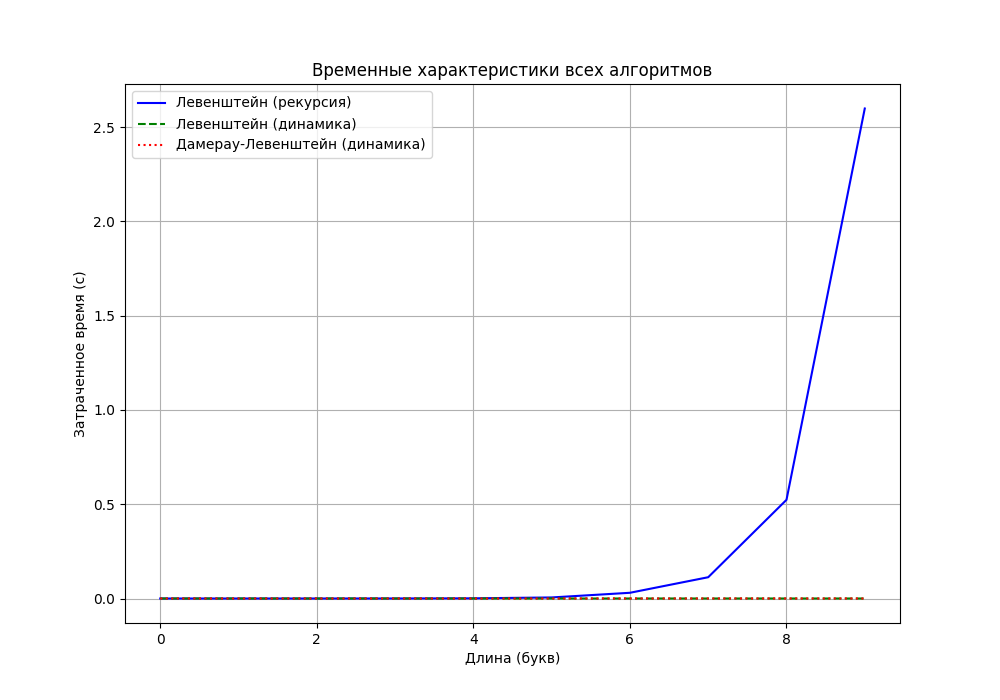
\includegraphics[width=0.8\linewidth]{img/Figure_3.png}
    \vspace{5mm}
    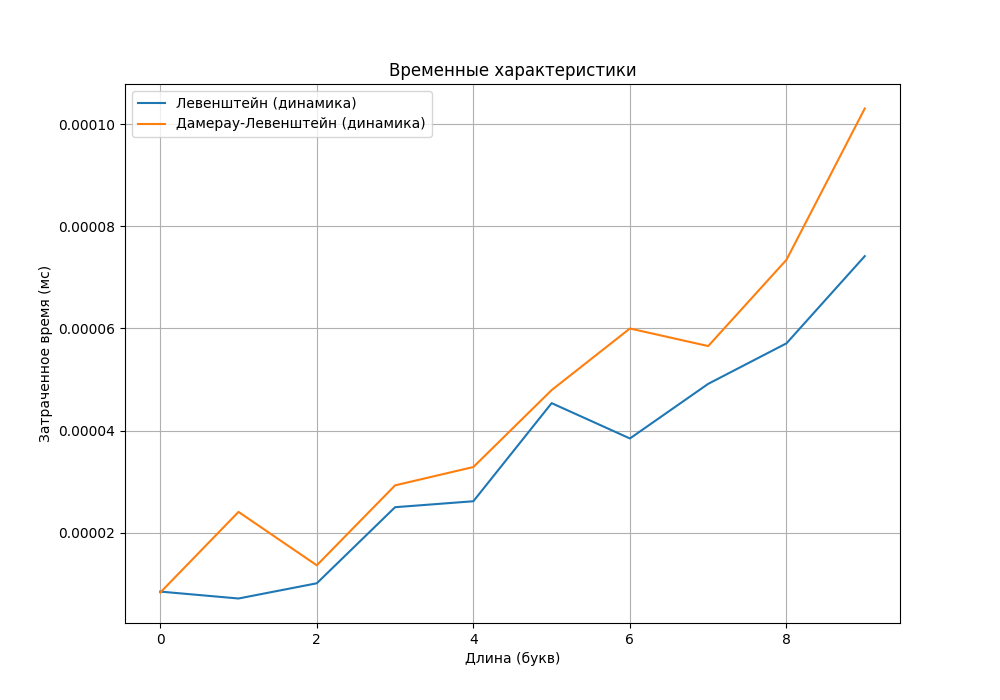
\includegraphics[width=0.8\linewidth]{img/Figure_2.png}
    \caption{Сравнение алгоритмов по времени}
    \label{fig:time_measurements}
\end{figure}


\clearpage


Наиболее эффективными являются алгоритмы, использующие динамический подход (матрицу), так как в рекурсивных алгоритмах большое количество повторных расчетов.

\section{Вывод}

Рекурсивный алгоритм, вычисляющий расстояние Левенштейна, работает по времени на несколько порядков дольше, чем динамический вариант (на 3-буквенных словах: в 10 раз; на 8-буквенных строках: в 10000 раз). Также стоит заметить, что динамические алгоритмы вычисления расстояний Левенштейна и Дамерау-Левенштейна сопостовимы между собой по времени выполнения и примерно равны.

Анализ расхода памяти показывает, что рекурсивный алгоритм имеет меньшие требования к памяти по сравнению с алгоритмом, использующим динамическое программирование. В случае динамического варианта алгоритма, считающего расстояние Дамерау-Левенштейна, несмотря на добавление операции перестановки, потребление памяти остается на уровне алгоритма, считающего расстояние Левенштейна, так как не требуется дополнительное пространство для хранения результатов перестановок.